\documentclass[12pt,a4paper]{report}
\usepackage{amsmath}
\usepackage{amsfonts}
\usepackage{amssymb}
\usepackage{fullpage}
\usepackage[slovak]{babel}
\usepackage[utf8]{inputenc}
\usepackage[T1]{fontenc}
\usepackage{fullpage}
\usepackage{indentfirst}
\usepackage{array}
\usepackage{graphicx}
\usepackage{caption}
\DeclareGraphicsExtensions{.png,.jpg}

\begin{document}
\begin{titlepage}
\centering\bfseries
		Fakulta matematiky, fyziky a informatiky\\Univerzita Komenského v Bratislave	
	\vspace*{\stretch{2.0}}

	\fontsize{23}{28}\textbf{Špecifikácia požiadaviek na softvér}\\
	\vspace*{\stretch{0.05}}
	\fontsize{16}{22}\textbf{Predikcia šírenia infekčných ochorení}\\
	\vspace*{\stretch{0.2}}
	\large\textit{Matúš Čongrády\\Tibor Hanesz\\Jonatan Foltyn\\Katarína Šimnová}

	\vspace*{\stretch{2.0}}
\end{titlepage}\bigskip
	\setcounter{tocdepth}{9}
	\tableofcontents
	
\renewcommand{\chaptername}{}	
\chapter[Analýza technológií, dekompozícia a dátový model]{\rmfamily\bfseries
	Analýza technológií, dekompozícia a dátový model}
	

\section[Možné použité technológie a postupy]{\rmfamily\bfseries
	Možné použité technológie a postupy}

\subsection[Technológie]{\rmfamily\bfseries
	Technológie}
Na strane servera sme sa rozhodli použiť server nginx a PHP. Nginx preto, lebo nie je tak robustný, je stále pravidelne podporovaný a taktiež nezávislý od jedného operačného systému. PHP sme zvolili kvôli jednoduchosti, ľahkému nasadeniu, osobnej preferencie a skúsenosti a vzhľadom na jednoduchosť nie je potrebné hľadieť na rýchlosť do detailov. Na čítanie súborov z excelu použijeme voľne dostupnú knižnicu PHPExcel.
\par
Na strane klienta použije HTML5 a CSS3 na layout. Okrem toho použijeme JavaScript a knižnicu jQuery spolu s nadstavbou pre validáciu pre komfortnejšie užívateľské rozhranie. Tieto technológie sme zvolili vzhľadom na rozšírenosť, osobnú preferenciu a skúsenosť. 
\par
Na vykreslenie mapy použijeme Google Map API v3. Je to najrozšírenejšie maps API, ktoré nám ponúka presne tú funkcionalitu, ktorú potrebujeme.
\pagebreak

\section[Deployment diagram]{\rmfamily\bfseries
	Deployment diagram}
Prichádzajúce HTTP požiadavky vyhodnotí najprv nginx server a následne PHP. Posiela statický obsah ako HTML, CSS, JavaScript a obrázky. Taktiež posiela dáta na vytvorenie animácie prostredníctvom métody POST.
\begin{figure}[htb]
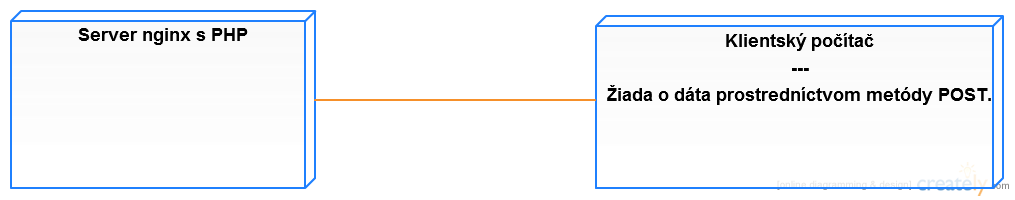
\includegraphics[scale=0.5]{deployment}
\caption[Deployment diagram]{Deployment diagram}
 \label{fig:Deployment diagram}
\end{figure}


\section[Domain model diagram]{\rmfamily\bfseries
	Domain model diagram}
Administrátor (zadávateľ) uploadne na stránku .xls súbor, ktorý server spracuje, a uloží si z neho dáta. Štruktúra uloženého údaju - počet ochorených / deň / kraj Slovenska. Server spracuje požiadavky od užívateľa a pošle statický obsah stránky. Webová stránka následne zobrazí animáciu pre užívateľa.
\begin{figure}[htb]
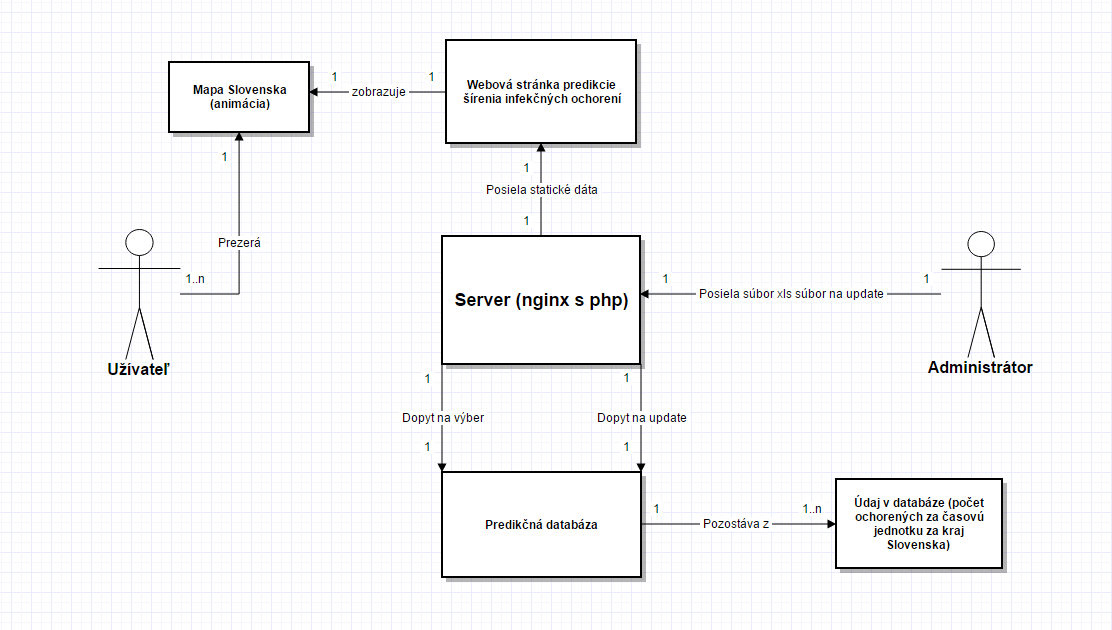
\includegraphics[scale=0.5]{Domain_model_diagram}
\caption[Domain model diagram]{Domain model diagram}
 \label{fig:Domain model diagram}
\end{figure}

\section[Data model]{\rmfamily\bfseries
	Data model}
Administrátor (zadávateľ) uploadne na stránku .xls alebo .xlsx súbor, ktorý server spracuje. Server dáta prekonvertuje do formátu json. Následne ich uloží do .json súboru, ktorý sa nachádza na serveri. Relatívna cesta k súboru: ../data/data.json
\begin{figure}[htb]
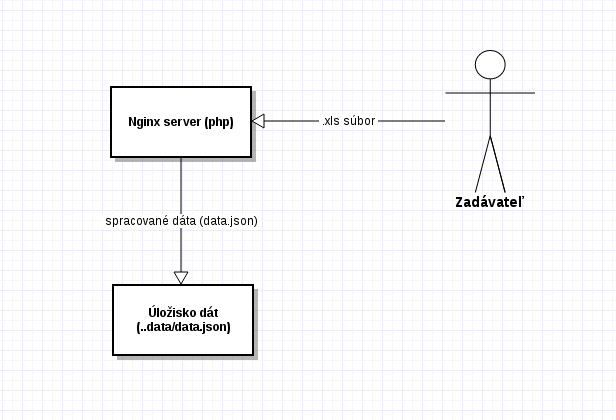
\includegraphics[scale=0.5]{data_model}
\caption[Data model]{Data model}
 \label{fig:Data model}
\end{figure}


\end{document}